\newpage

\section{Additional Results from Chapter 3 Case Study 1}

This appendix recreates Figures \ref{fig:sens_spec} and \ref{fig:viterbi_dives_D26b} from the first case study of Chapter 3 for $\alpha = 0,0.025,0.049,0.525,1$. The results for $\alpha = 0.025$ and $\alpha = 0.525$ are very similar to those for $\alpha = 0.049$, but I include them here for completeness.

\begin{figure}[H]
    \centering
    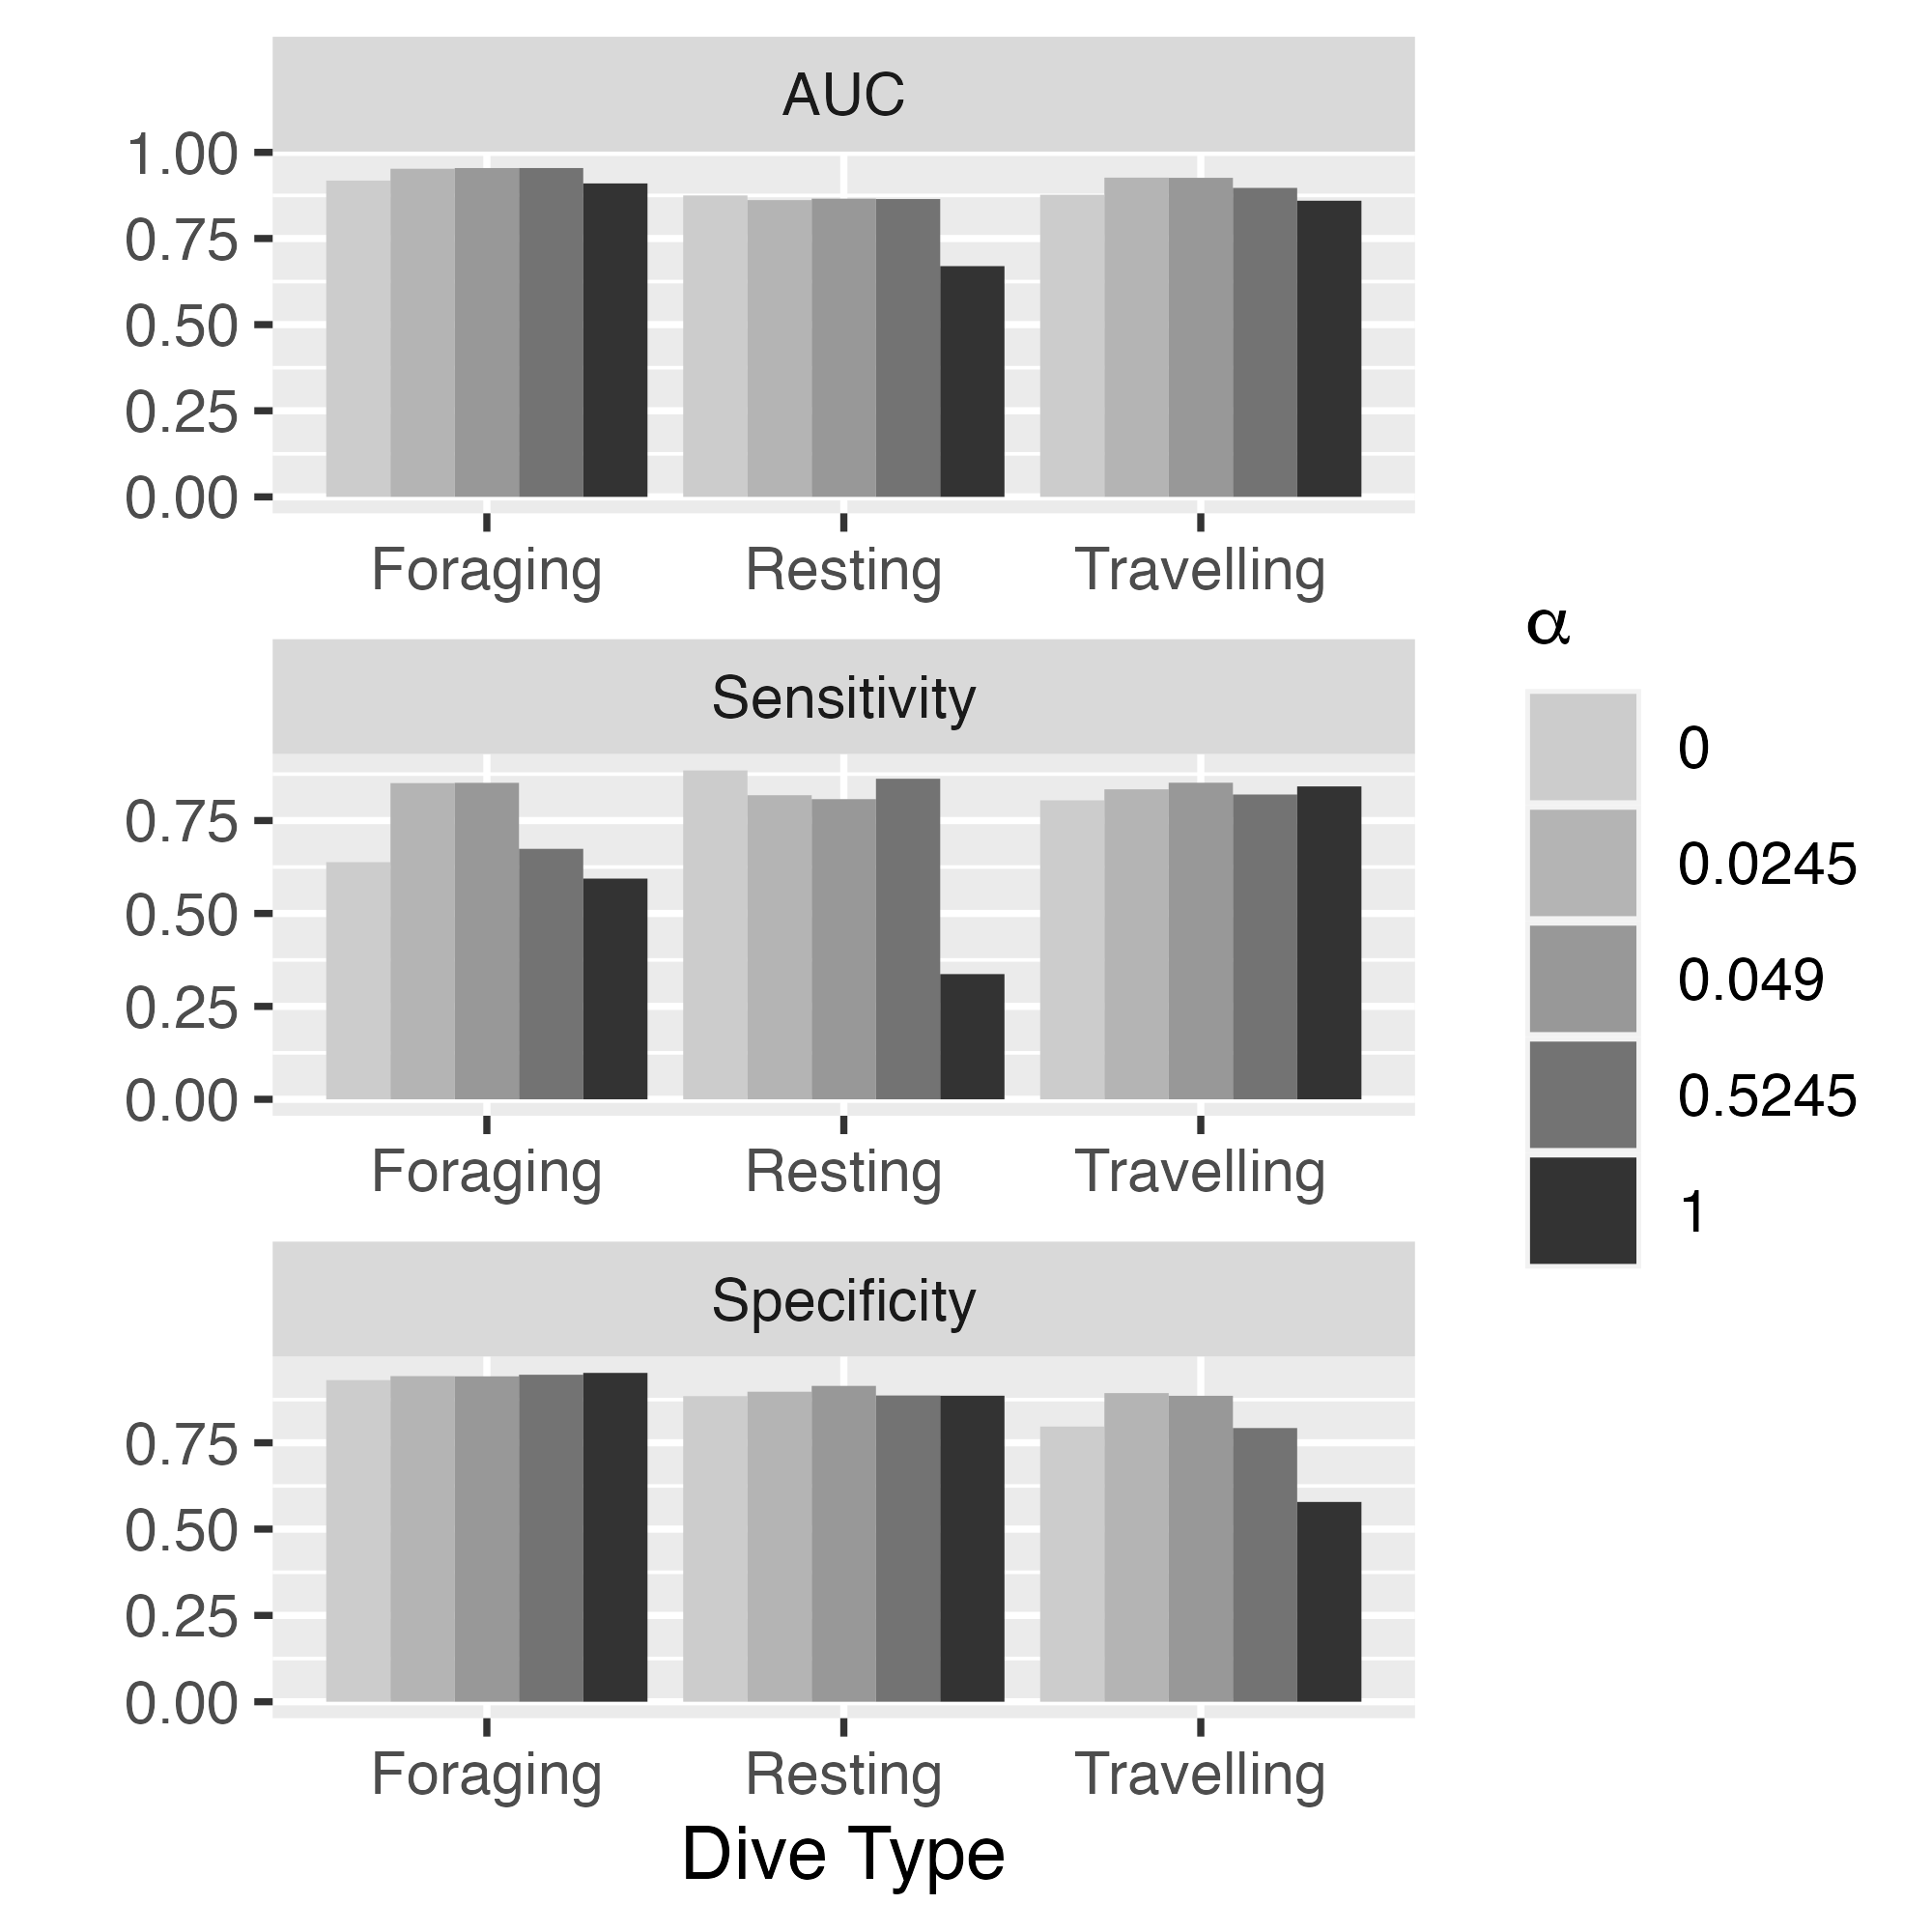
\includegraphics[width=4in]{body_chapters/chap_3/plt/1-1-1-logMDDD_all_model_comparison_all_alphas.png}
    \caption[Sensitivity, specificity, and AUC values associated with each dive type from the first case study.]{Sensitivity, specificity, and AUC values associated with each dive type. True values are determined via the drone-detected dive types. The PHMMs for each value of $\alpha$ were fit using the entire dataset with a selected sub-profile held out. Then, the dives for that sub-profile were estimated by using the forward-backward algorithm on the sub-profile with the drone-detected labels removed. I repeated this process for every sub-profile to get a full set of estimated dive types.}
    \label{fig:sens_spec_app}
\end{figure}

\begin{figure}[H]
    \centering
    \begin{subfigure}[t]{0.45\textwidth}
        \centering
        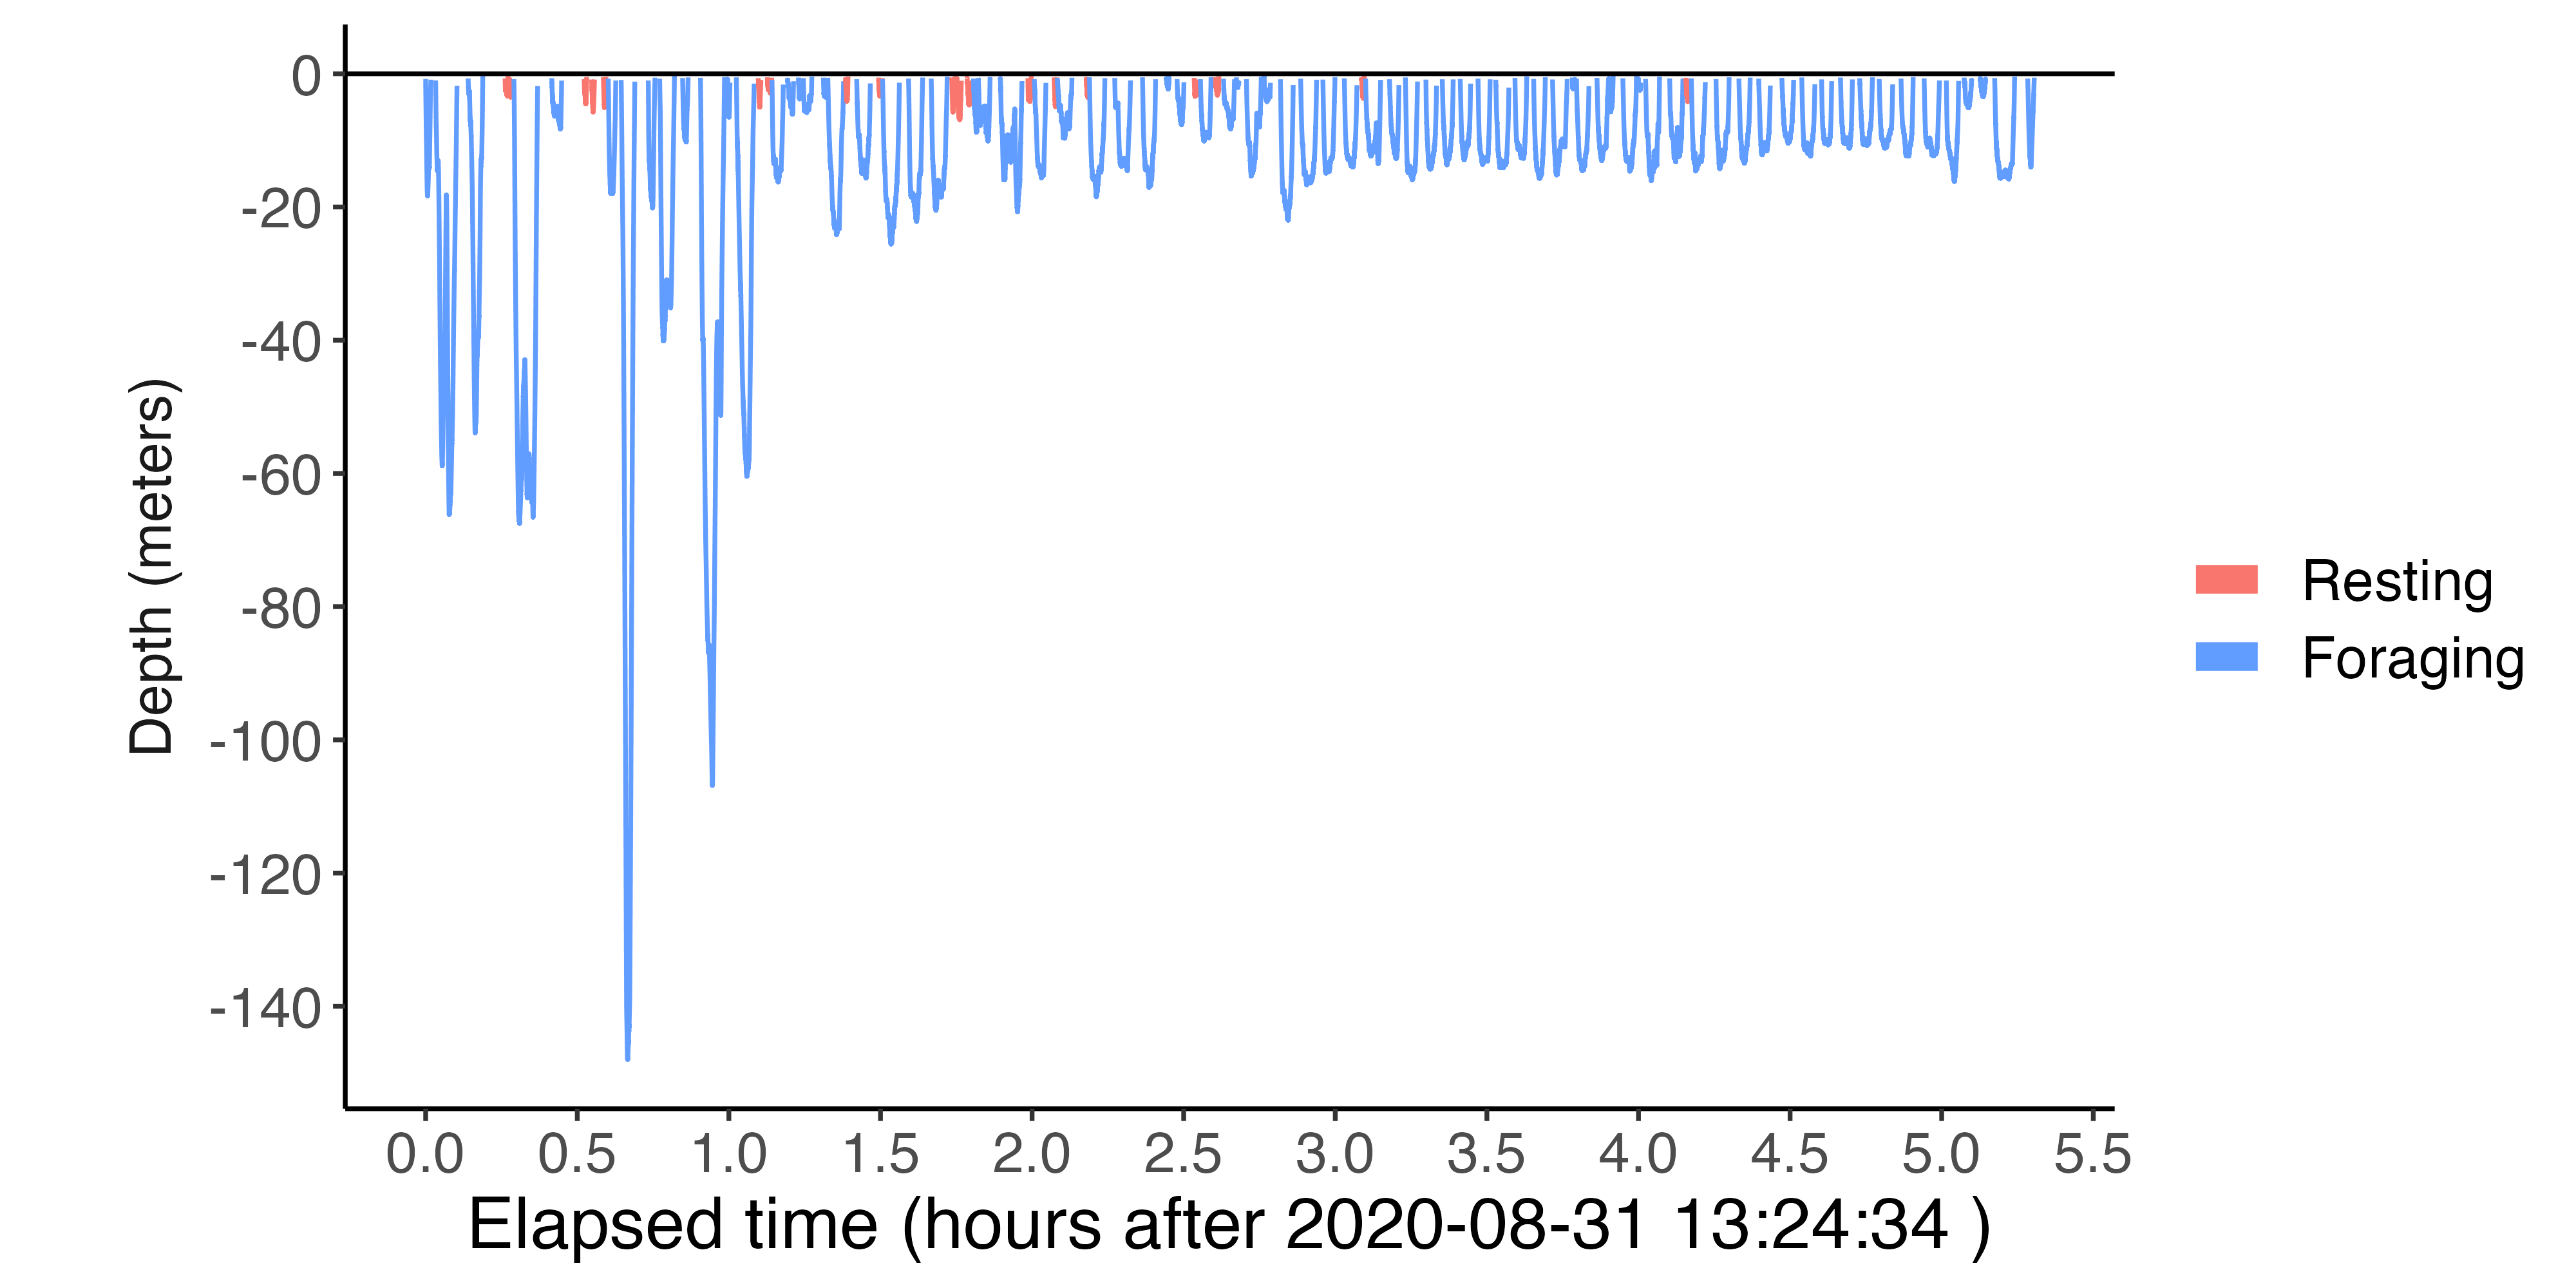
\includegraphics[width = 2.7in]{body_chapters/chap_3/plt/D26b-profile-D26b-fixed-1.png}
        \caption{Decoded dives for PHMM with $\alpha = 1.000$ (the ``natural" weighting).}
    \end{subfigure}
    ~ 
    \begin{subfigure}[t]{0.45\textwidth}
        \centering
        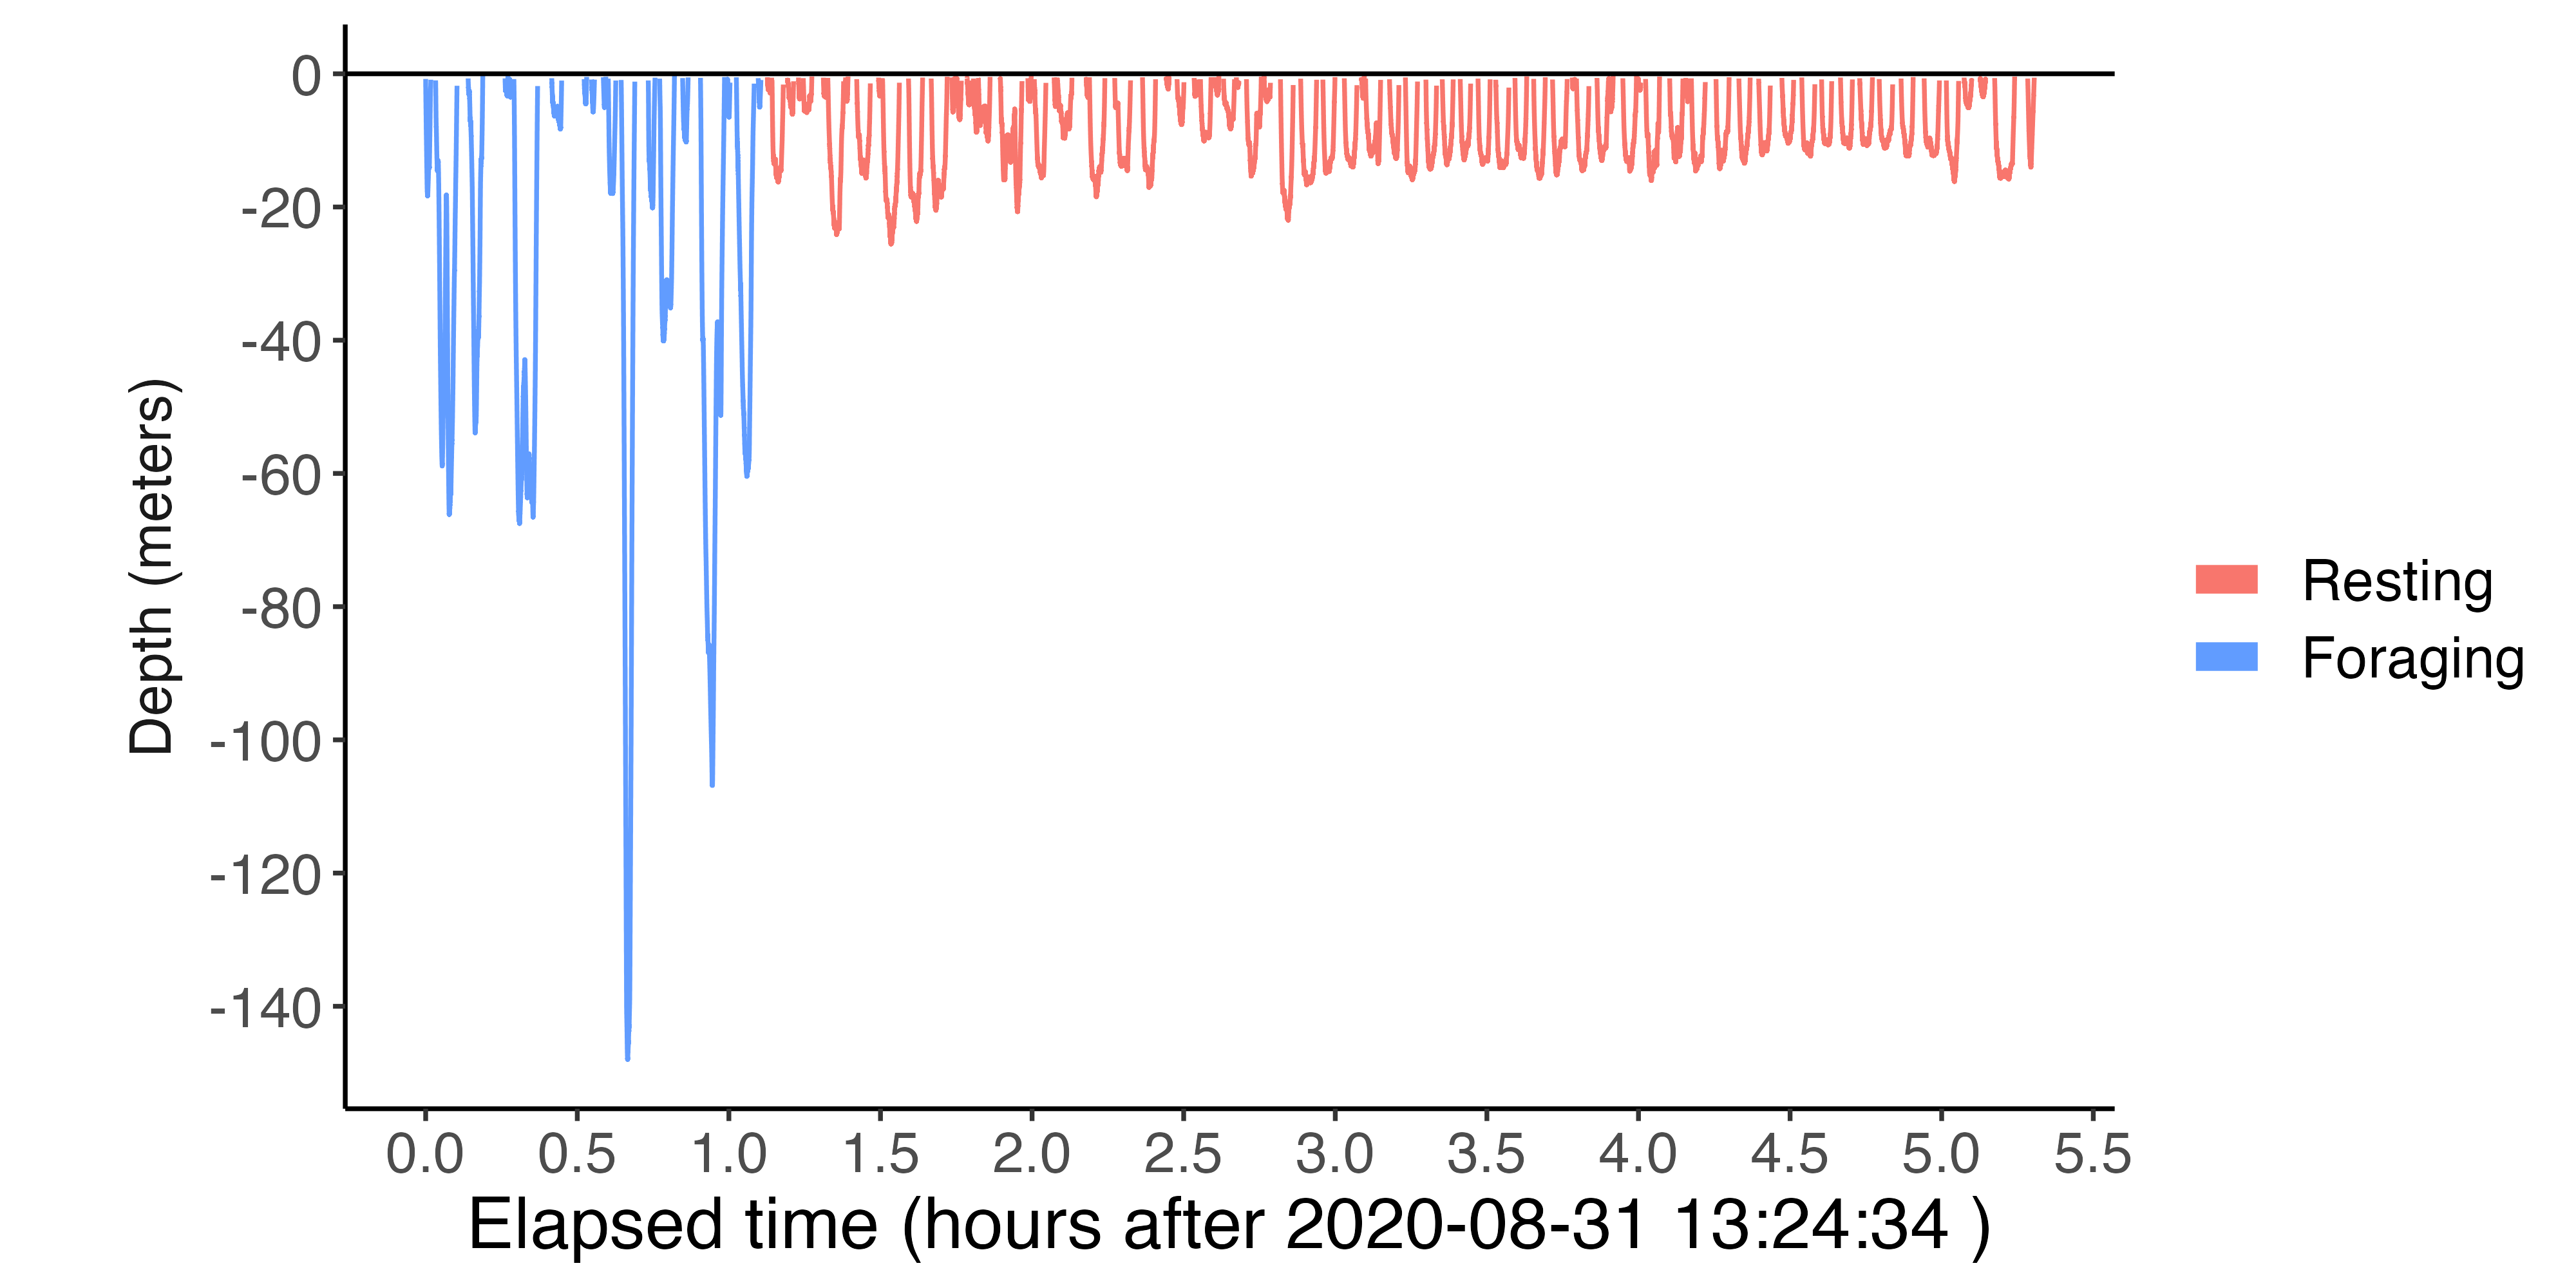
\includegraphics[width = 2.7in]{body_chapters/chap_3/plt/D26b-profile-D26b-fixed-0.5245.png}
        \caption{Decoded dives for PHMM with $\alpha = 0.525$.}
    \end{subfigure}
    \\
    \begin{subfigure}[t]{0.45\textwidth}
        \centering
        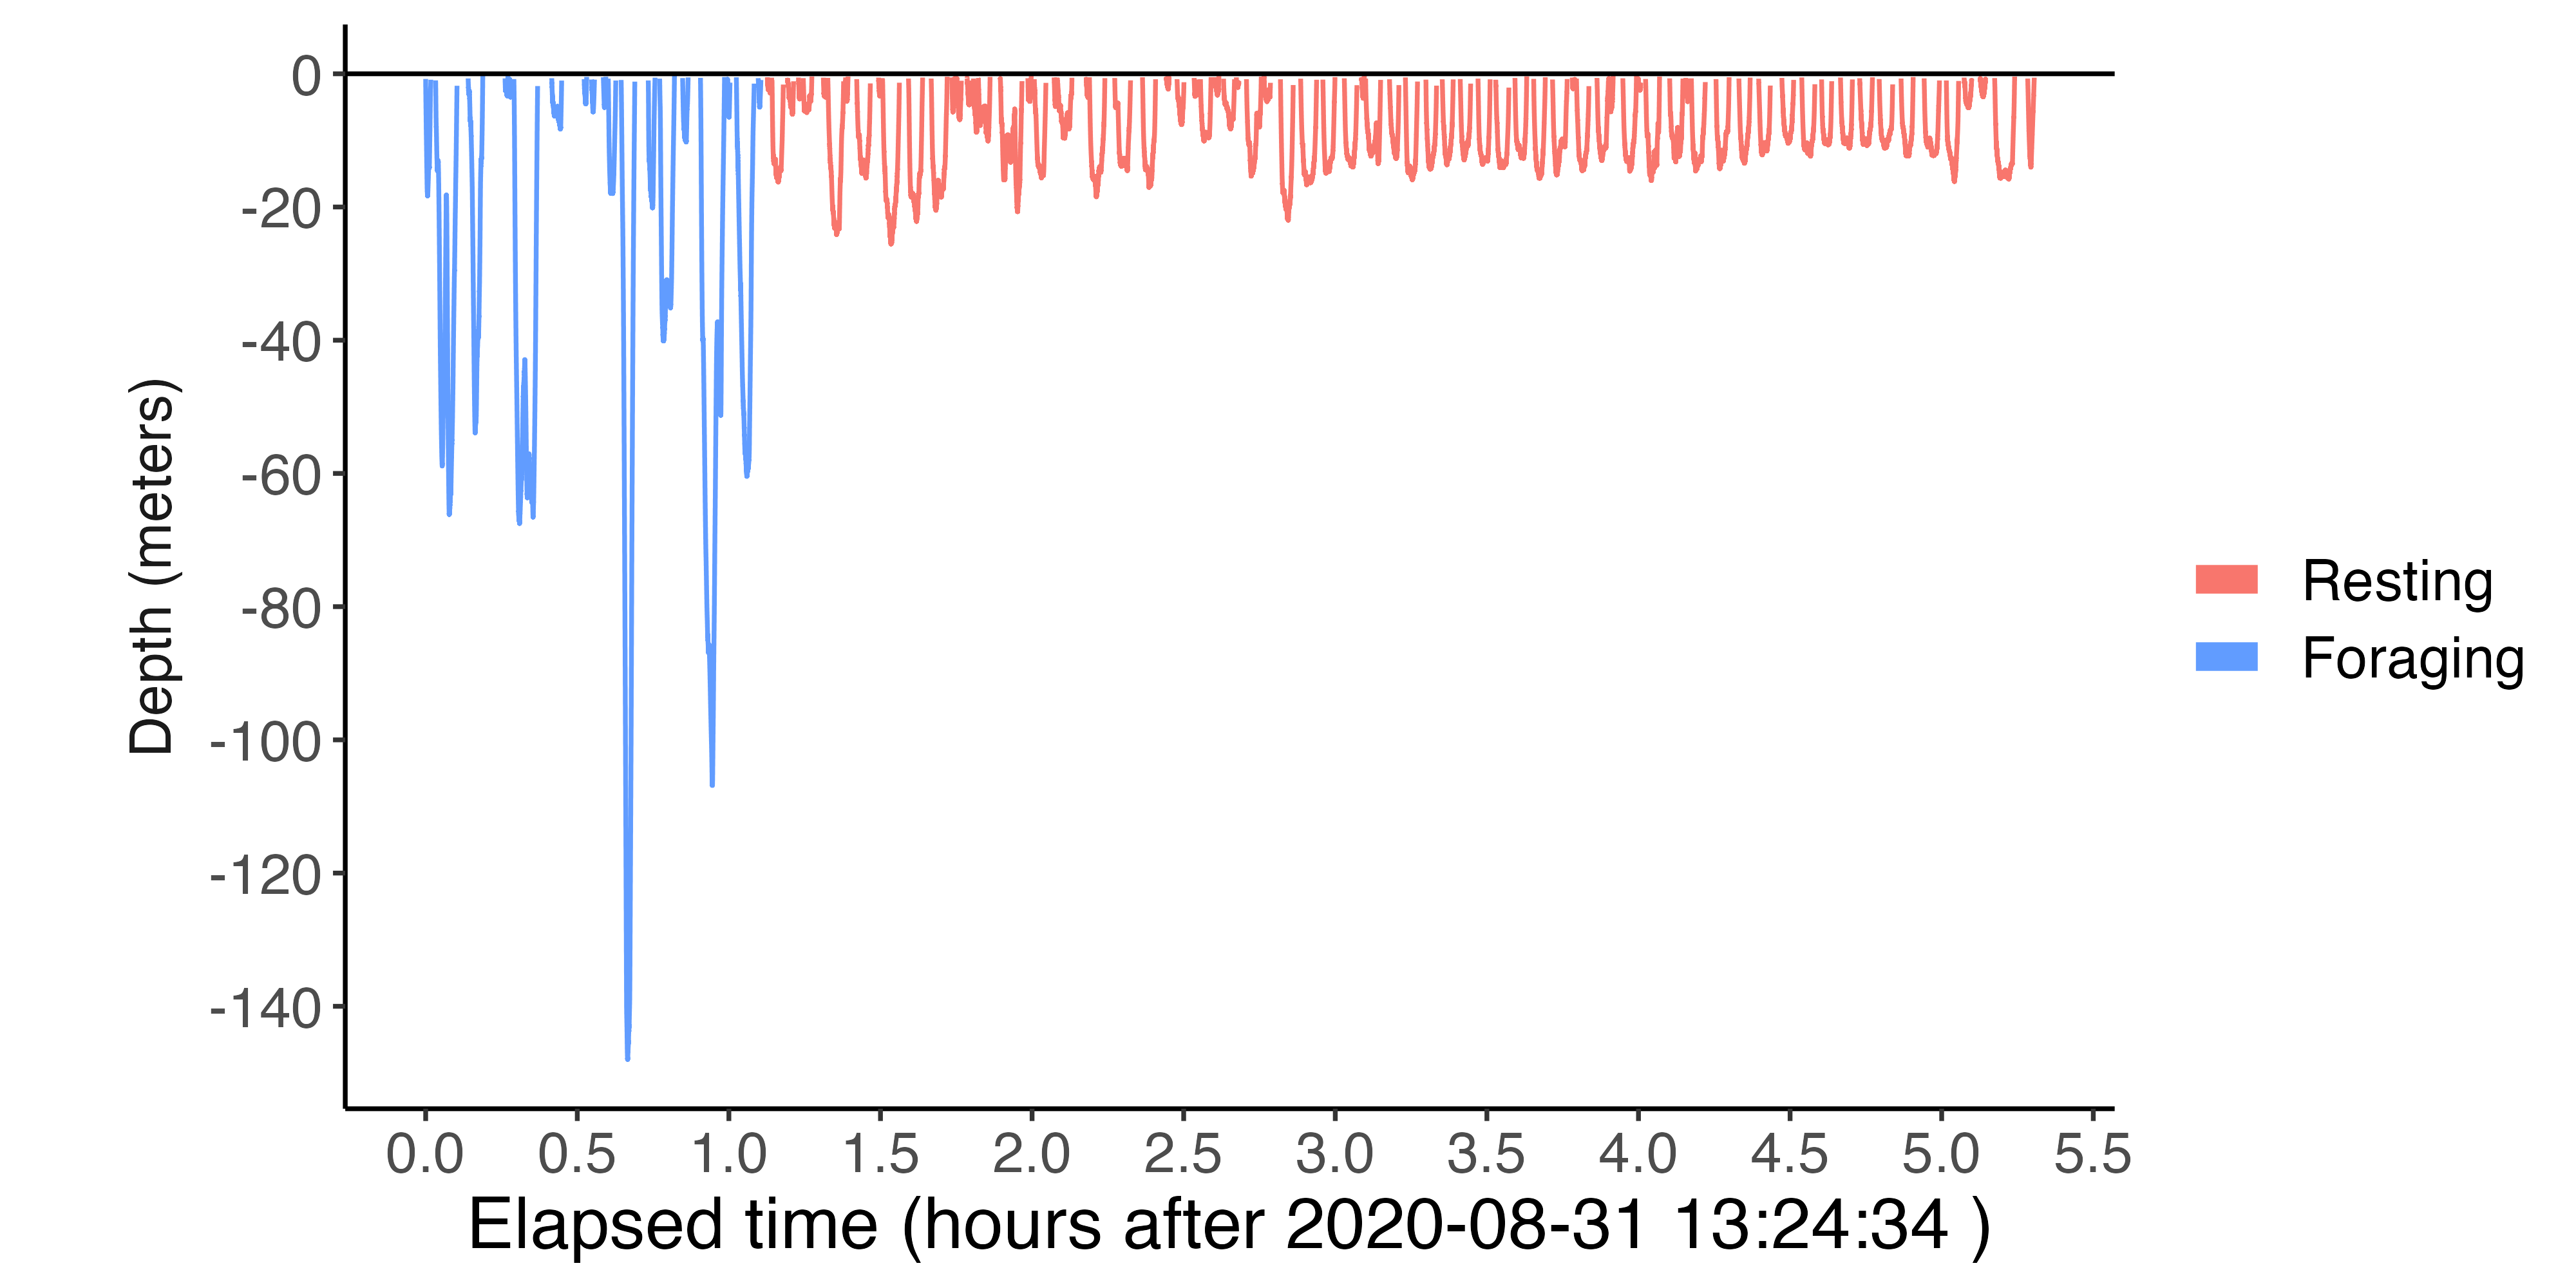
\includegraphics[width = 2.7in]{body_chapters/chap_3/plt/D26b-profile-D26b-fixed-0.049.png}
        \caption{Decoded dives for PHMM with $\alpha = 0.049$.}
    \end{subfigure}
    ~
    \begin{subfigure}[t]{0.45\textwidth}
        \centering
        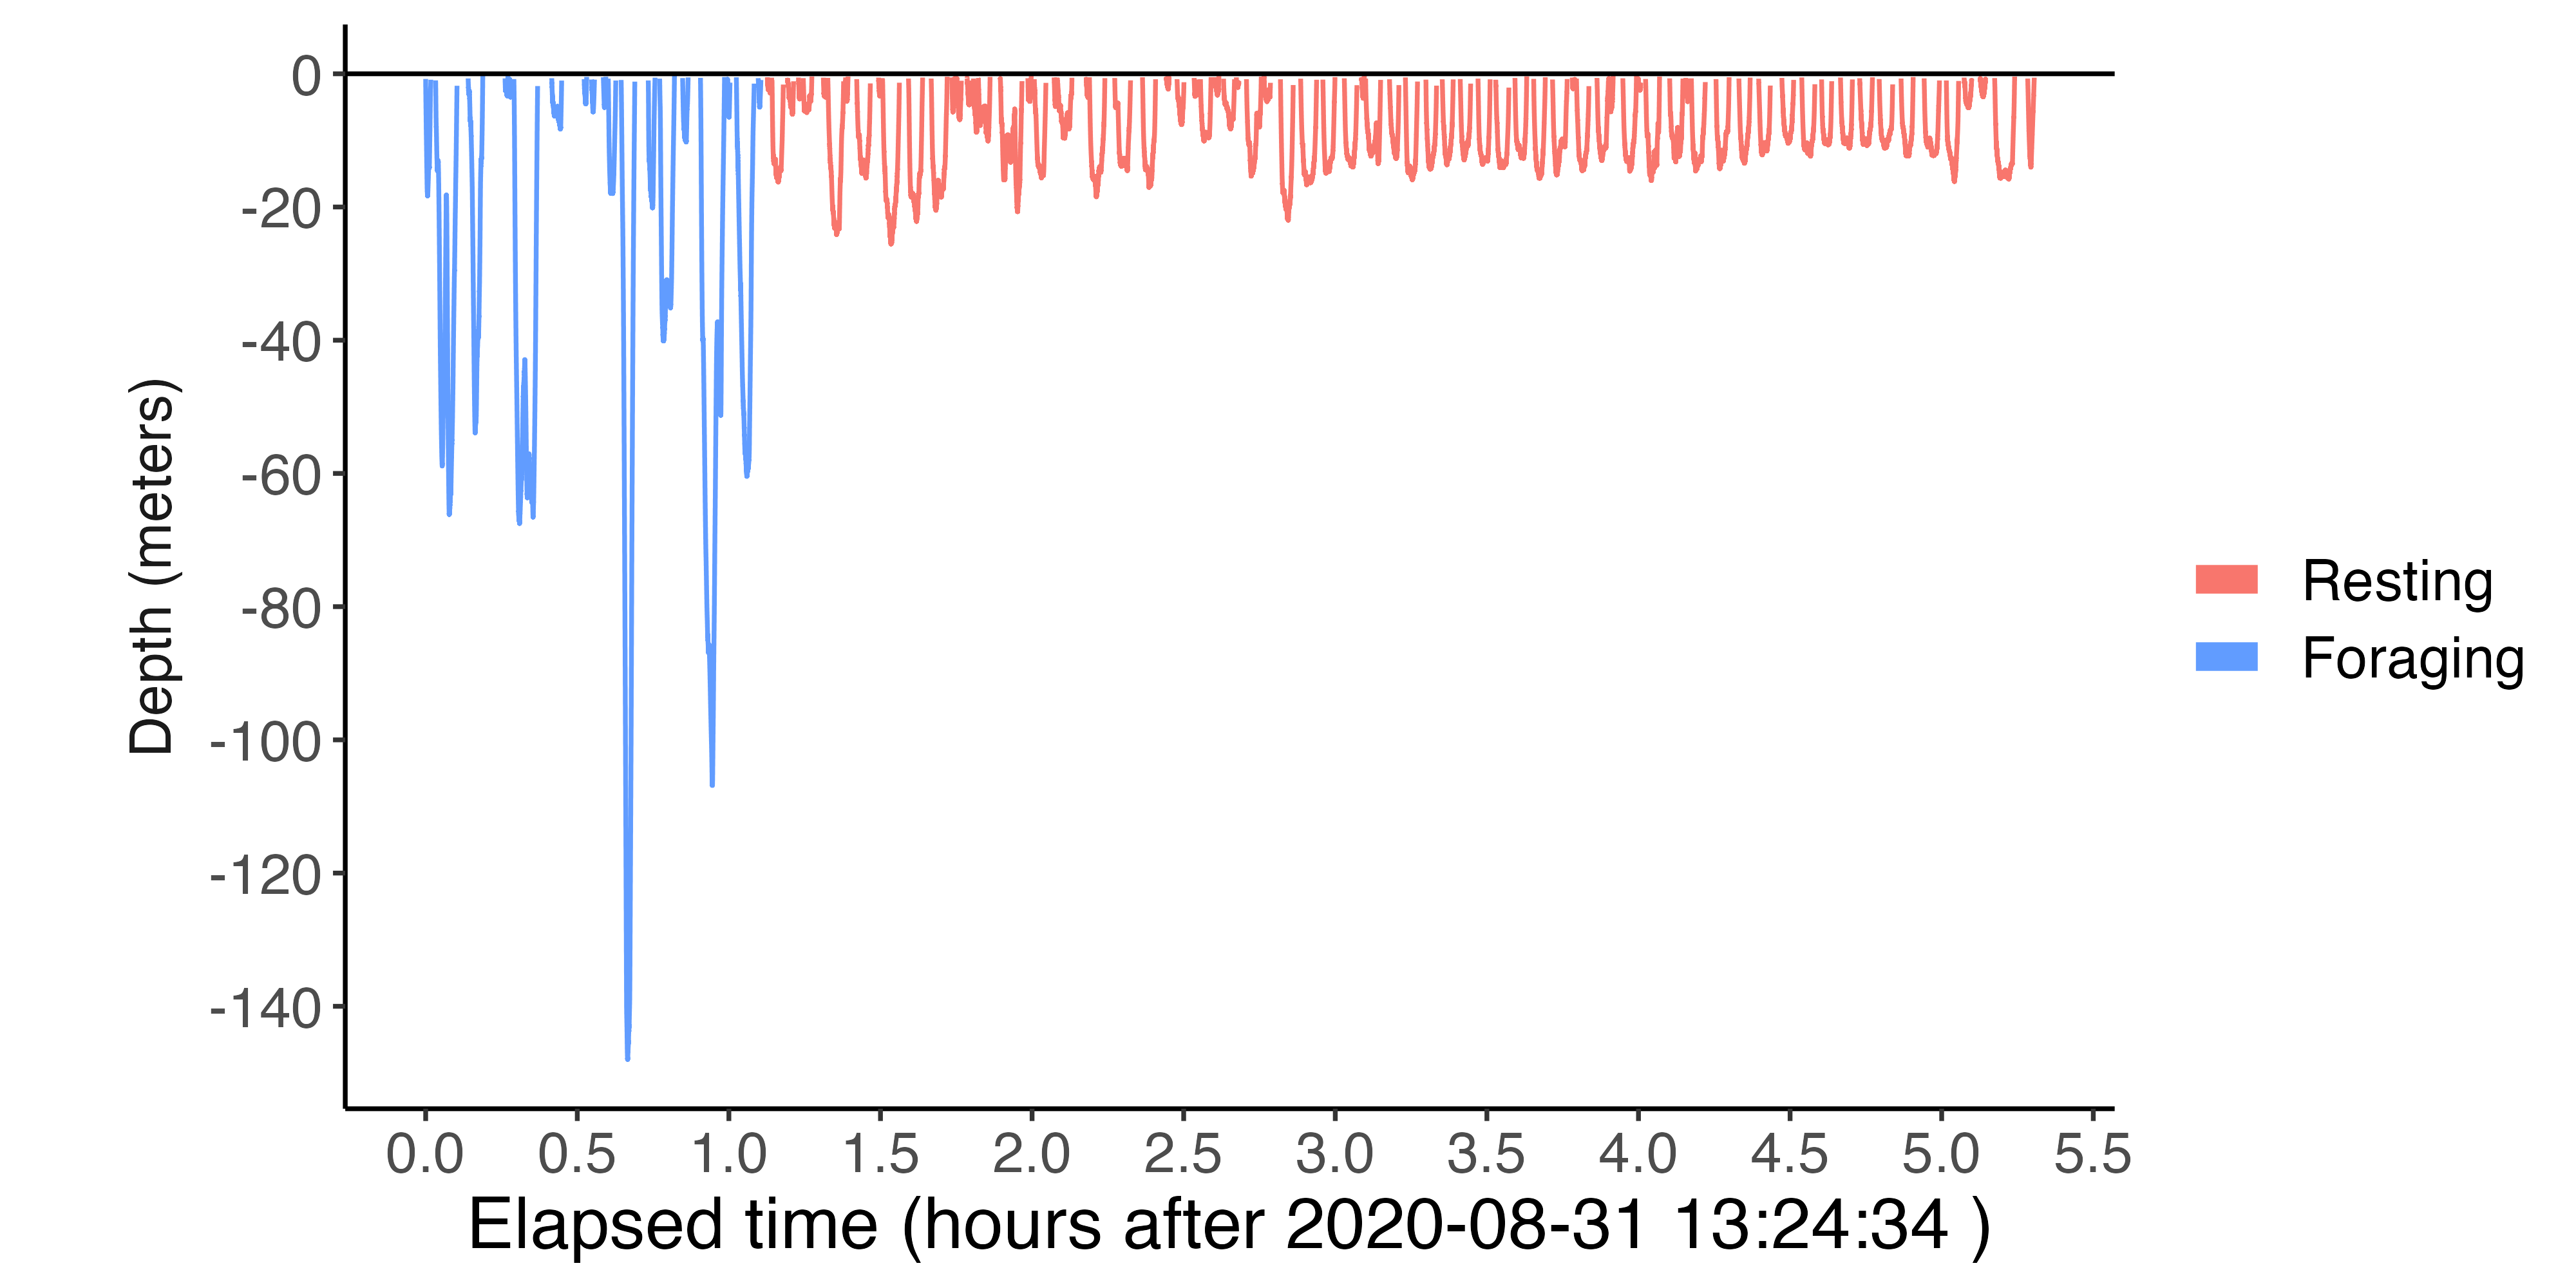
\includegraphics[width = 2.7in]{body_chapters/chap_3/plt/D26b-profile-D26b-fixed-0.0245.png}
        \caption{Decoded dives for PHMM with $\alpha = 0.025$.}
    \end{subfigure}
    \\
    \begin{subfigure}[t]{0.45\textwidth}
        \centering
        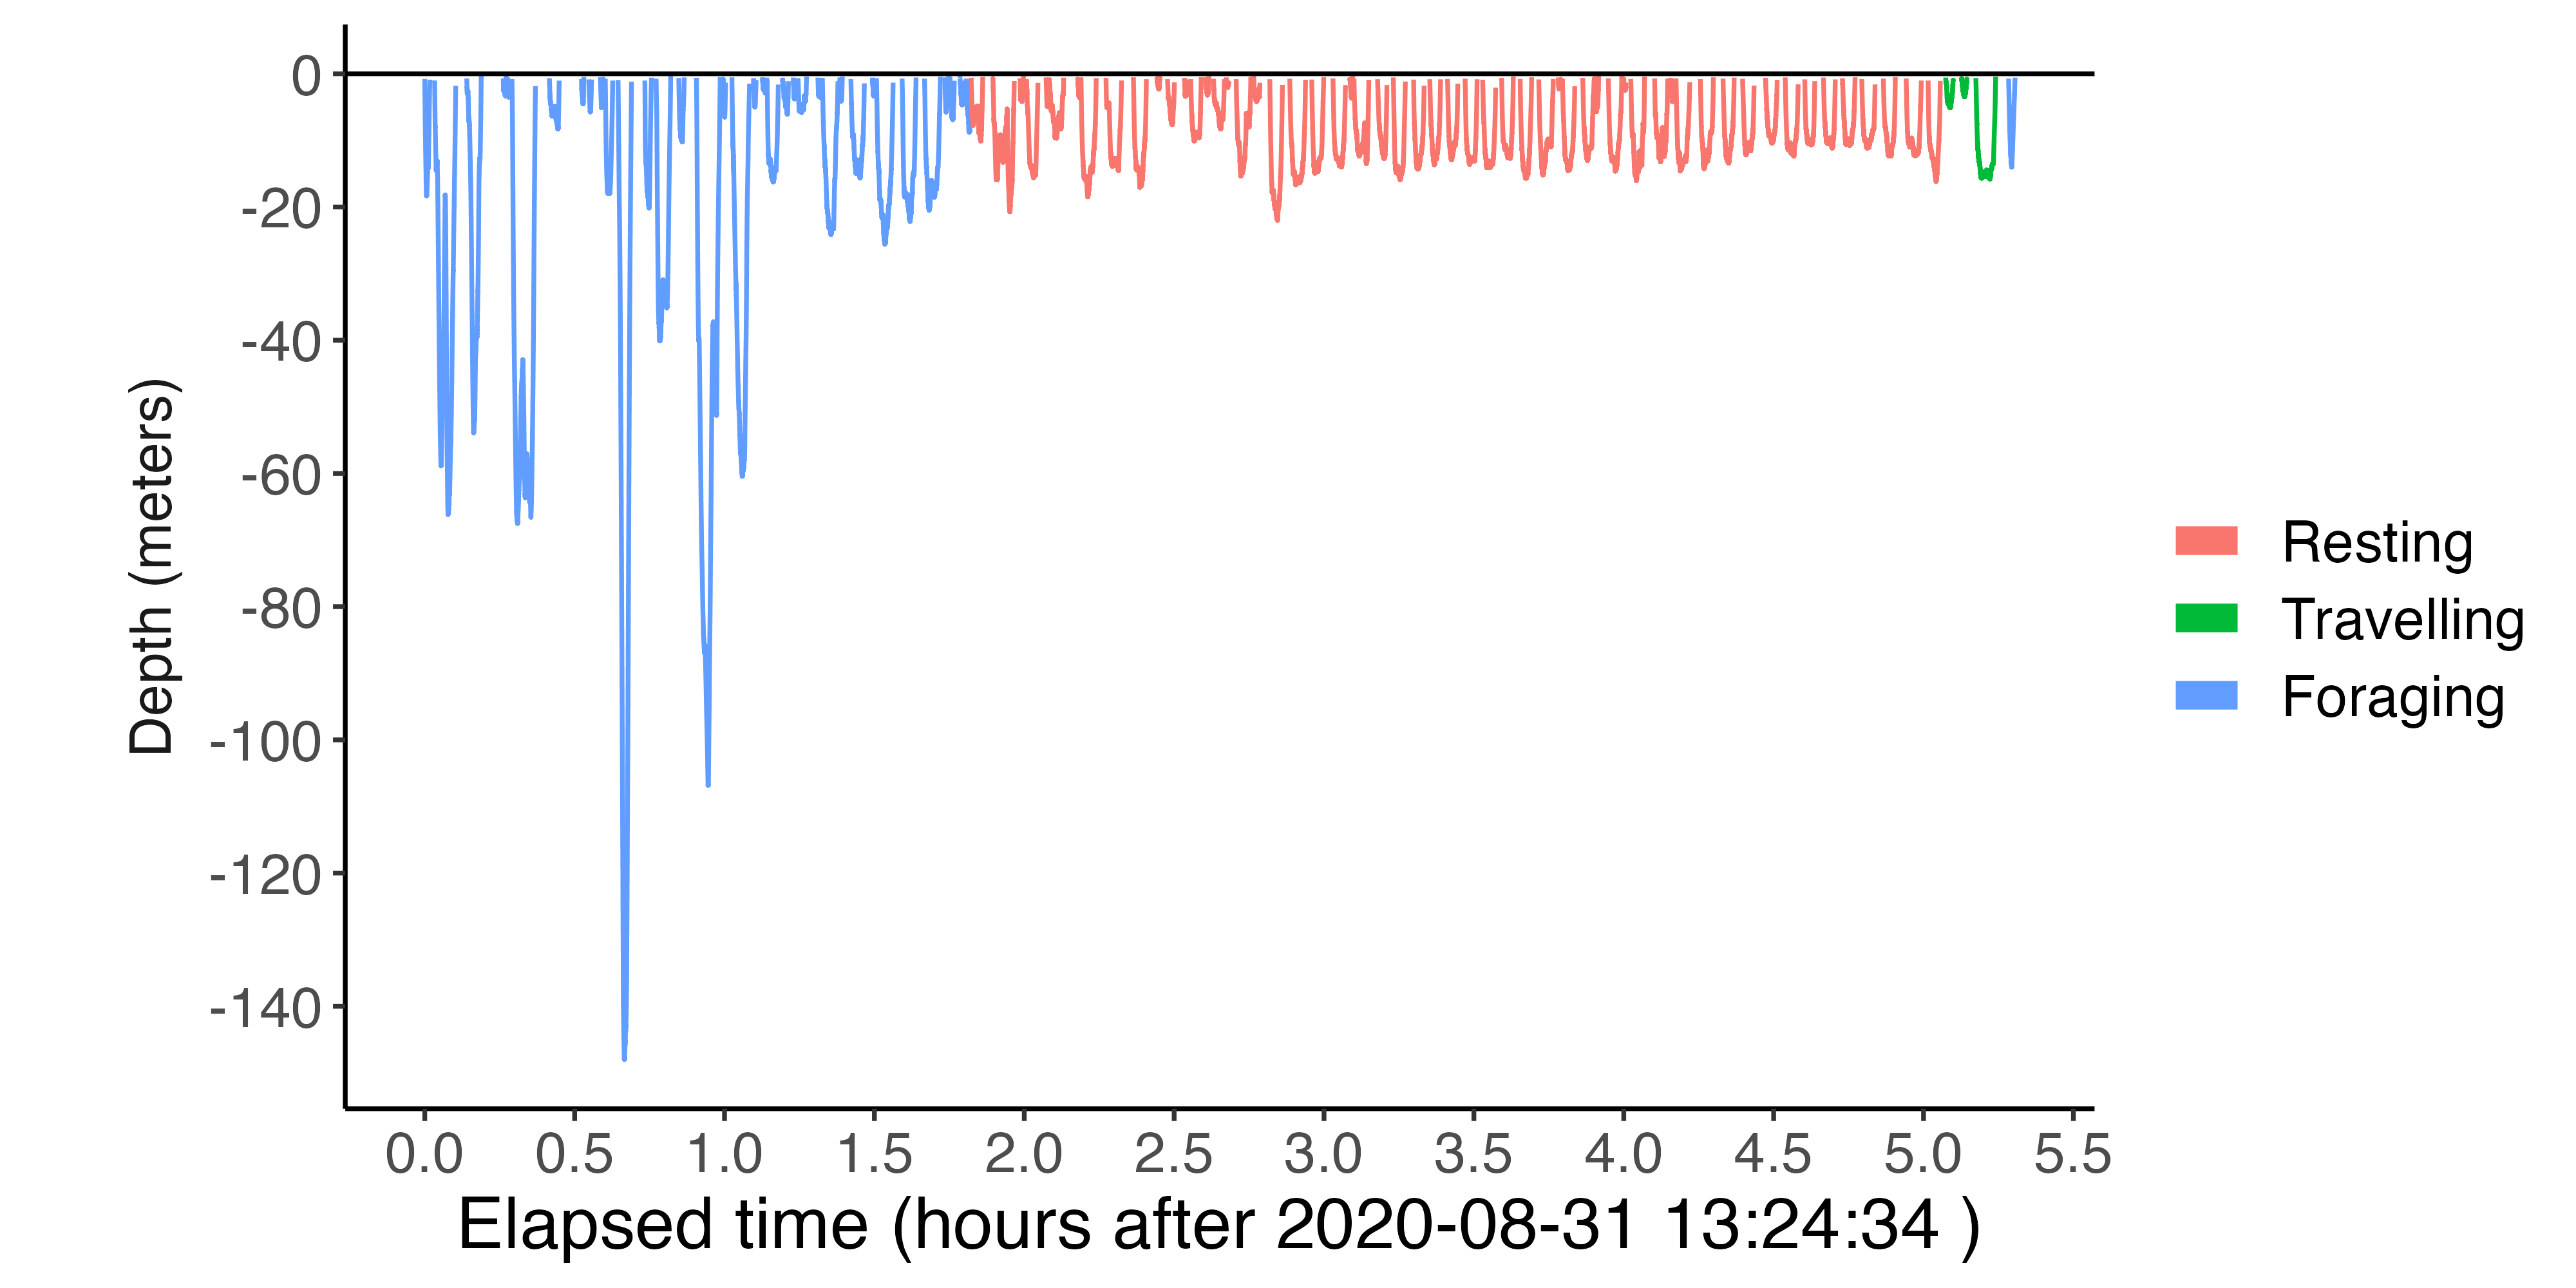
\includegraphics[width = 2.7in]{body_chapters/chap_3/plt/D26b-profile-D26b-fixed-0.png}
        \caption{Decoded dives for PHMM with $\alpha = 0.000$ (treating the unlabelled observations as missing).}
    \end{subfigure}
    ~
    \begin{subfigure}[t]{0.45\textwidth}
        \centering
        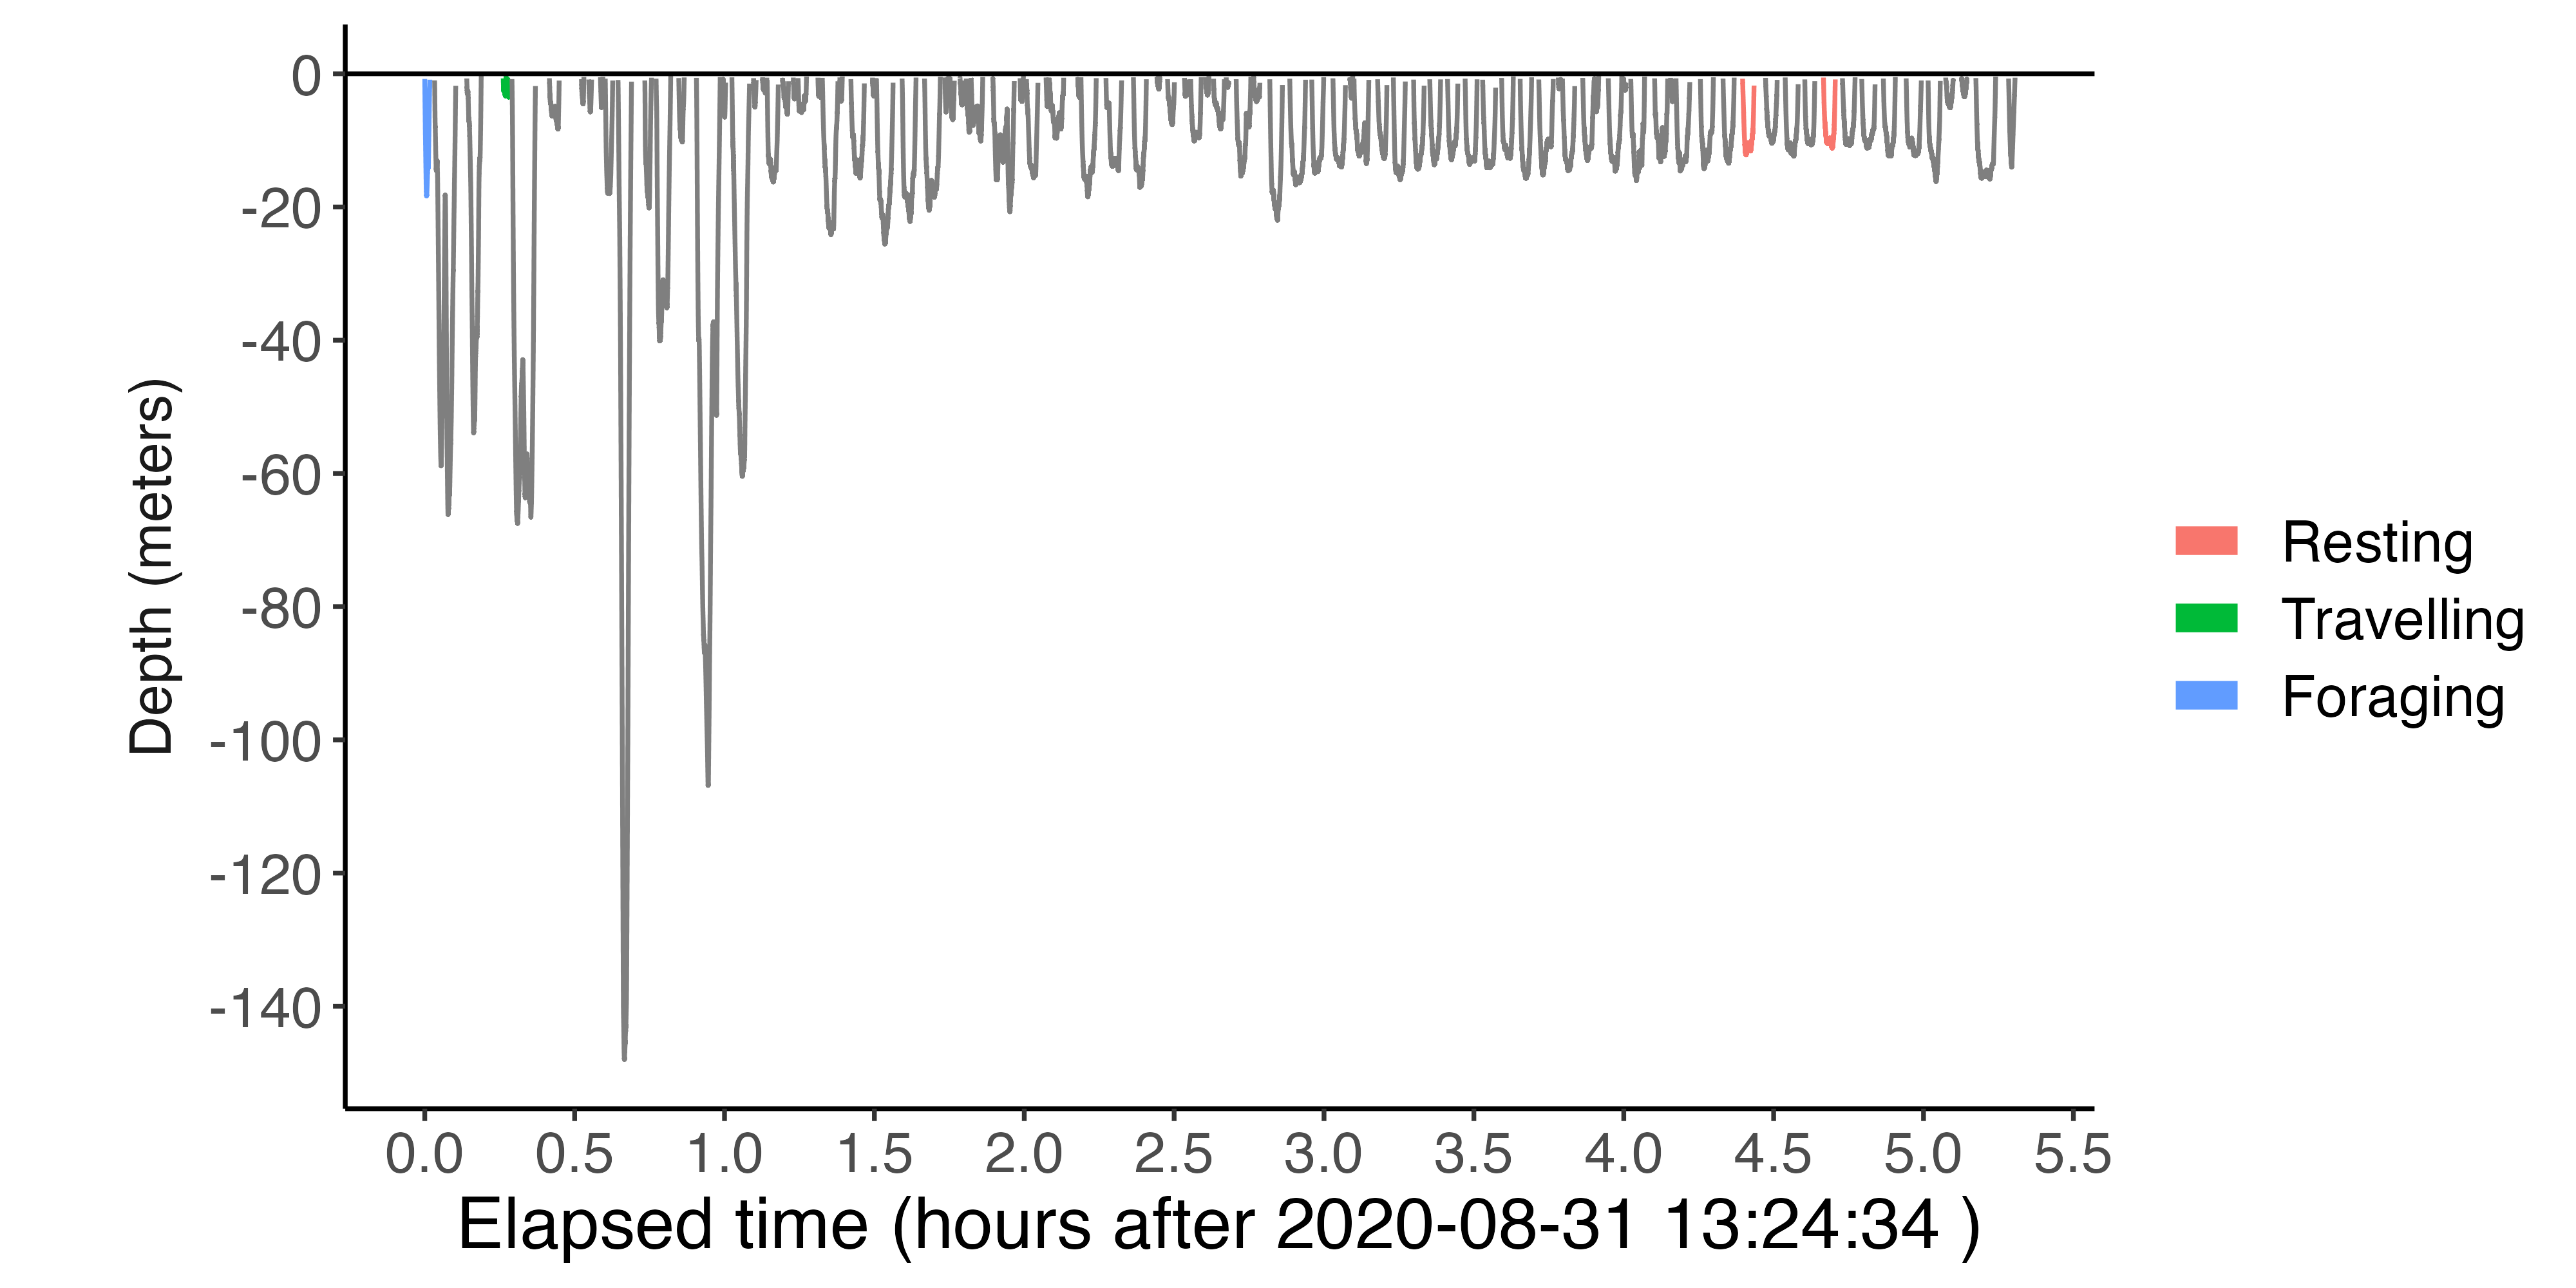
\includegraphics[width = 2.7in]{body_chapters/chap_3/plt/D26b-profile-D26b-known_states.png}
        \caption{Dive profile with true drone-detected labels.}
    \end{subfigure}
    \caption[Viterbi-decoded dives for a given sub-profile and several different PHMMs.]{Viterbi-decoded dives for a given sub-profile and several different PHMMs. Each PHMM was fit to the dataset with the sub-profile held out. Then the Viterbi algorithm was used on the held-out dataset with its labels removed in order to test the predictive performance of each PHMM.}
    \label{fig:viterbi_dives_D26b_app}
\end{figure}